%*********************************************************
% Federal University of Santa Catarina (UFSC)
% 
% Author: 				Gabriel Mariano Marcelino
% 
% Created on: 			13/12/2017
% Last modification: 	15/12/2017
%*********************************************************

\documentclass[12pt]{book}

\usepackage[a4paper,left=2.5cm,right=2.5cm,top=2.5cm,bottom=2.5cm]{geometry}
\usepackage[T1]{fontenc}  
\usepackage[utf8]{inputenc} 
\usepackage[english]{babel}
\usepackage{ae}
\usepackage{graphicx}
\usepackage[hidelinks]{hyperref}
\usepackage{fancyhdr}
\usepackage{subfigure}
\usepackage{nomencl}				% Nomenclature list
\usepackage{float}
\usepackage{titlesec}
\usepackage{booktabs}
\usepackage{emptypage}
\usepackage{lettrine}				% First letter bigger in the begining of a chapter
\usepackage{tabularx}
\usepackage{enumitem}				% Custom enumerate

\title{Telemetry, Tracking and Command Module of the FloripaSat Project}
\author{Gabriel Mariano Marcelino}
\date{13/12/2017}

% File metadata
\hypersetup
{
    pdfauthor	={Gabriel Mariano Marcelino},
    pdfsubject	={Telemetry, Tracking and Command Module Documentation},
    pdftitle	={Telemetry, Tracking and Command Module of the FloripaSat Project},
    pdfkeywords	={Cubesats, TTCs, Telecomunications}
}

% URLs font style
\urlstyle{same}

% First chapter page style
\titleformat{\chapter}[display]
	{\bfseries\Large}
	{\filright\MakeUppercase{\chaptertitlename} \Large\thechapter}
	{1ex}
	{\titlerule\vspace{1ex}\filleft}
	[\vspace{1ex}\titlerule]

% Header style
\pagestyle{fancy}
\fancyhf{}
\fancyhead[RO]{Telemetry, Tracking and Command Module}
\fancyhead[LE]{\nouppercase{\leftmark}}
\fancyfoot[RO]{\thepage}
\fancyfoot[LE]{\thepage}
\renewcommand{\footrulewidth}{0.5pt} 

% List of abbreviations
\makenomenclature
\setlength\nomlabelwidth{2cm}

% Bibliography style
\bibliographystyle{unsrt}

% Table cell size limit and alignment
\newcolumntype{L}[1]{>{\raggedright\arraybackslash}p{#1}}
\newcolumntype{C}[1]{>{\centering\arraybackslash}p{#1}}
\newcolumntype{R}[1]{>{\raggedleft\arraybackslash}p{#1}}

\begin{document}

\begin{titlepage}

%****************************************************
%****************************************************
%-- TITLE PAGE --------------------------------------
%****************************************************
%****************************************************
\thispagestyle{empty}

\begin{flushleft}
FLORIPASAT - TTC-DOC - REV1
\end{flushleft}

\begin{figure}[!ht]
	\begin{flushleft}
		
\includegraphics[width=5cm]{figures/floripasat.png}
	\end{flushleft}
\end{figure}

\begin{flushleft}
\Huge{\textbf{Telemetry, Tracking and Command Module of the FloripaSat Project}}
\rule[0pt]{\textwidth}{5pt}
\end{flushleft}

\vspace{0.2cm}

\begin{flushleft}
\textit{Module Documentation} \\
\textit{GSE, Federal University of Santa Catarina, Florianópolis - Brazil}
\end{flushleft}

\vfill
\vfill

\begin{flushright}
December 2017
\end{flushright}

\pagenumbering{roman}
\setcounter{page}{1}

\end{titlepage}

\cleardoublepage

%****************************************************
%****************************************************
%-- AUTHOR PAGE -------------------------------------
%****************************************************
%****************************************************

\thispagestyle{empty}

\begin{center}

\textbf{FloripaSat Project, Telemetry, Tracking and Command Module Documentation}

\textit{December, 2017}

\vspace{1cm}

\textbf{Project Manager:}

Eduardo Augusto Bezerra

\vspace{1cm}

\textbf{Author:}

Gabriel Mariano Marcelino

\vspace{1cm}

\textbf{Contributing Authors:}

Anselmo Luis da Silva Junior \\
Marcelo Daniel Berejuck \\
Sara Vega Martinez \\

\vspace{1cm}

\textbf{Layout:}

Gabriel Mariano Marcelino

\end{center}

\vspace{8cm}

\begin{figure}[!h]
%\begin{wrapfigure}{l}{0.25\textwidth}
	\begin{center}
		\includegraphics[width=0.25\textwidth]{figures/by-sa.eps}
	\end{center}
\end{figure}
%\end{wrapfigure}

\textcopyright\  2017 by Federal University of Santa Catarina. Telemetry, Tracking and Command Module of the FloripaSat Project. This work is licensed under the Creative Commons Attribution-ShareAlike 4.0 International License. To view a copy of this license, visit http://creativecommons.org/licenses/by-sa/4.0/.

%****************************************************
%****************************************************
%-- ABSTRACT ----------------------------------------
%****************************************************
%****************************************************

\chapter*{Abstract}

This document...

\smallskip
\noindent \textbf{Keywords:} Cubesats. Embedded systems. Telecomunications.

%****************************************************
%****************************************************
%-- TABLE OF CONTENTS -------------------------------
%****************************************************
%****************************************************
\tableofcontents

%****************************************************
%****************************************************
%-- LIST OF FIGURES ---------------------------------
%****************************************************
%****************************************************

\listoffigures
\addcontentsline{toc}{chapter}{List of Figures}

%****************************************************
%****************************************************
%-- LIST OF TABLES ----------------------------------
%****************************************************
%****************************************************

\listoftables
\addcontentsline{toc}{chapter}{Lista of Tables}

%****************************************************
%****************************************************
%-- NOMENCLATURE ---------------------------
%****************************************************
%****************************************************

\printnomenclature
\addcontentsline{toc}{chapter}{Nomenclature}

%****************************************************
%****************************************************
%-- INTRODUCTION ------------------------------------
%****************************************************
%****************************************************

\chapter{Introduction}

\pagenumbering{arabic}

\lettrine{I}{ntroduction}...

\nomenclature{\textbf{TTC}}{Telemetry, Tracking and Command.}
\nomenclature{\textbf{PCB}}{Printed Circuit Board.}
\nomenclature{\textbf{USB}}{Universal Serial Bus.}

\cite{site}.

\section{Module Requirements}

In the list below, the TTC module requirements for the mission are described. These requirements are nominated as TMR\nomenclature{\textbf{TMR}}{Telemetry, Tracking and Command Module Requirements.}, or Telemetry, Tracking and Command Module Requirements.

\begin{enumerate}[label=\textit{TMR \arabic*}, leftmargin=*, align=left]
	\item The FloripaSat shall have a physical device to inhibit radio frequency (RF\nomenclature{\textbf{RF}}{Radio Frequency.}) transmission.
	
	\begin{footnotesize}
		Compliance with CDS\nomenclature{\textbf{CDS}}{CubeSat Design Specification.} 3.3.9: The use of three independent inhibits is highly recommended and can reduce required documentation and analysis.	
	\end{footnotesize}
	
	\item The CubeSat will have the RF power output to the transmitting antenna input no greater than 1,5 W.
	
	\begin{footnotesize}
		Compliance with CDS 3.3.9.1.
	\end{footnotesize}
	
	\item The CubeSat will have the RF power output to the transmitting antenna input no less than 1,0 W (or 30 dBm).
	
	\begin{footnotesize}
		Defined by team analysis.
	\end{footnotesize}
	\item No CubeSats shall generate or transmit any RF signal from the time of integration into the P-POD\nomenclature{\textbf{P-POD}}{Poly-Picosatellite Orbital Deployer.} through 45 minutes after on-orbit deployment from the P-POD.
	
	\begin{footnotesize}
		Compliance with CDS.
	\end{footnotesize}
	
	\item TTC transceiver shall transmit and receive on the frequency of 437,9 Mhz.
	
	\begin{footnotesize}
		Defined by the team, based on available spectrum allocation to Amateur communication.
	\end{footnotesize}
	
	\item TTC beacon shall transmit on the frequency of 145,9 Mhz.
	
	\begin{footnotesize}
		Defined by the team, based on available spectrum allocation to Amateur communication.
	\end{footnotesize}
	
	\item TTC shall modulate and demodulate information using GFSK\nomenclature{\textbf{GFSK}}{Gaussian Frequency-Shift Keyring.}.
	
	\begin{footnotesize}
		Defined by the team.
	\end{footnotesize}
	
	\item TTC Beacon must transmit periodic beacon messages at an interval of 10
seconds, except when in hibernation or shutdown mode. Allows ground stations to track and receive satellite data even if telecommand was not sent to the satellite.
	\item TTC transceiver must receive signals from ground stations and demodulate them.
	\item TTC must interface with OBDH, exchanging encoded raw data received or to be transmitted.
	\item TTC must interface with OBDH using the SPI protocol ($@$2 KHz).
	
	\begin{footnotesize}
		Defined by the team.
	\end{footnotesize}
	
	\item TTC radio must modulate raw data received from OBDH using GFSK, prior to transmission, and demodulate received data and forward raw data to OBDH.
	\item TTC transceiver shall transmit and receive data at a baud rate of 2400 bps. Defined by the team, based on link budget analysis.
	\item TTC beacon shall transmit data at a baud rate of 1200 bps.
	
	\begin{footnotesize}
		Defined by the team, based on link budget analysis.
	\end{footnotesize}
	
	\item TTC beacon shall transmit packets using the NGHam and AX.25 protocols.
	
	\begin{footnotesize}
		Defined by the team.
	\end{footnotesize}
	
	\item A same beacon packet must be transmitted in both NGHam and AX.25 protocols.
	
	\begin{footnotesize}
		Defined by the team.
	\end{footnotesize}
	
	\item TTC must receive the batteries voltages from the EPS module at every 10 seconds.
	
	\begin{footnotesize}
		Defined by the team.
	\end{footnotesize}
	
	\item The payload from the packets transmitted by the beacon must contain at least the satellite ID ("FLORIPASAT") and batteries voltages (received from the EPS module at every 10 seconds).
	\item TTC uC must perform the antenna deployment of the VHF band antenna.
	
	\begin{footnotesize}
		Defined by the team.
	\end{footnotesize}
	
	\item Between the beacon packets transmissions, the beacon MCU and radio must operate in low power mode, to save energy.
	
	\begin{footnotesize}
		Defined by the team.
	\end{footnotesize}
	
	\item TTC PAs (Power amplifiers) must just only be activated during transmissions. When they are not in operation, they must be turned off.
	
	\begin{footnotesize}
		Defined by the team.
	\end{footnotesize}
	
	\item All the beacon critical data, like time control and antenna deployment status, must be stored in a non-volatile memory.
	
	\begin{footnotesize}
		Defined by the team.
	\end{footnotesize}
	
	\item TTC beacon must be able to receive a 24 hour shutdown command from the OBDH module.
	
	\begin{footnotesize}
		Compliance with AMSAT/IARU regulations.
	\end{footnotesize}
	
\end{enumerate}

%****************************************************
%****************************************************
%-- HARDWARE ----------------------------------------
%****************************************************
%****************************************************

\chapter{Hardware}

\lettrine{T}{he} TTC board is composed by the following main components:

\begin{itemize}
	\item MSP430F6659, as the beacon microcontroller.
	\item RF4463F30, as the radio module for the beacon and the telemetry link.
\end{itemize}

In the figure \ref{fig:ttc-board}, ...

\begin{figure}[!h]
	\begin{center}
		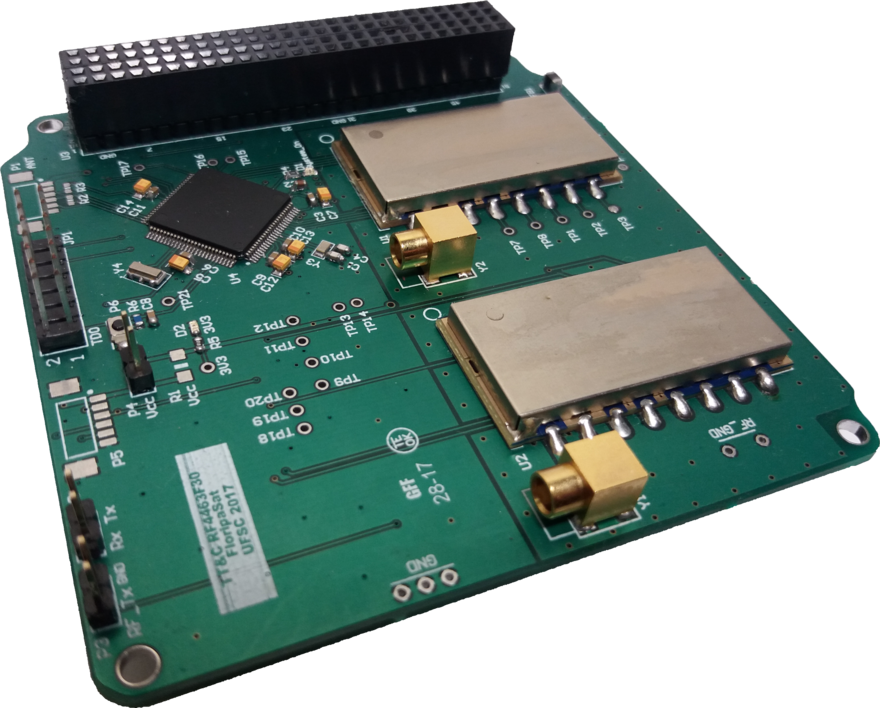
\includegraphics[width=0.75\textwidth]{figures/ttc_board.png}
		\caption{TTC PCB.}
		\label{fig:ttc-board}
	\end{center}
\end{figure}

\section{General Diagram}

In the figure \ref{fig:hardware-diagram}, a general hardware diagram can be seen.

\begin{figure}[!h]
	\begin{center}
		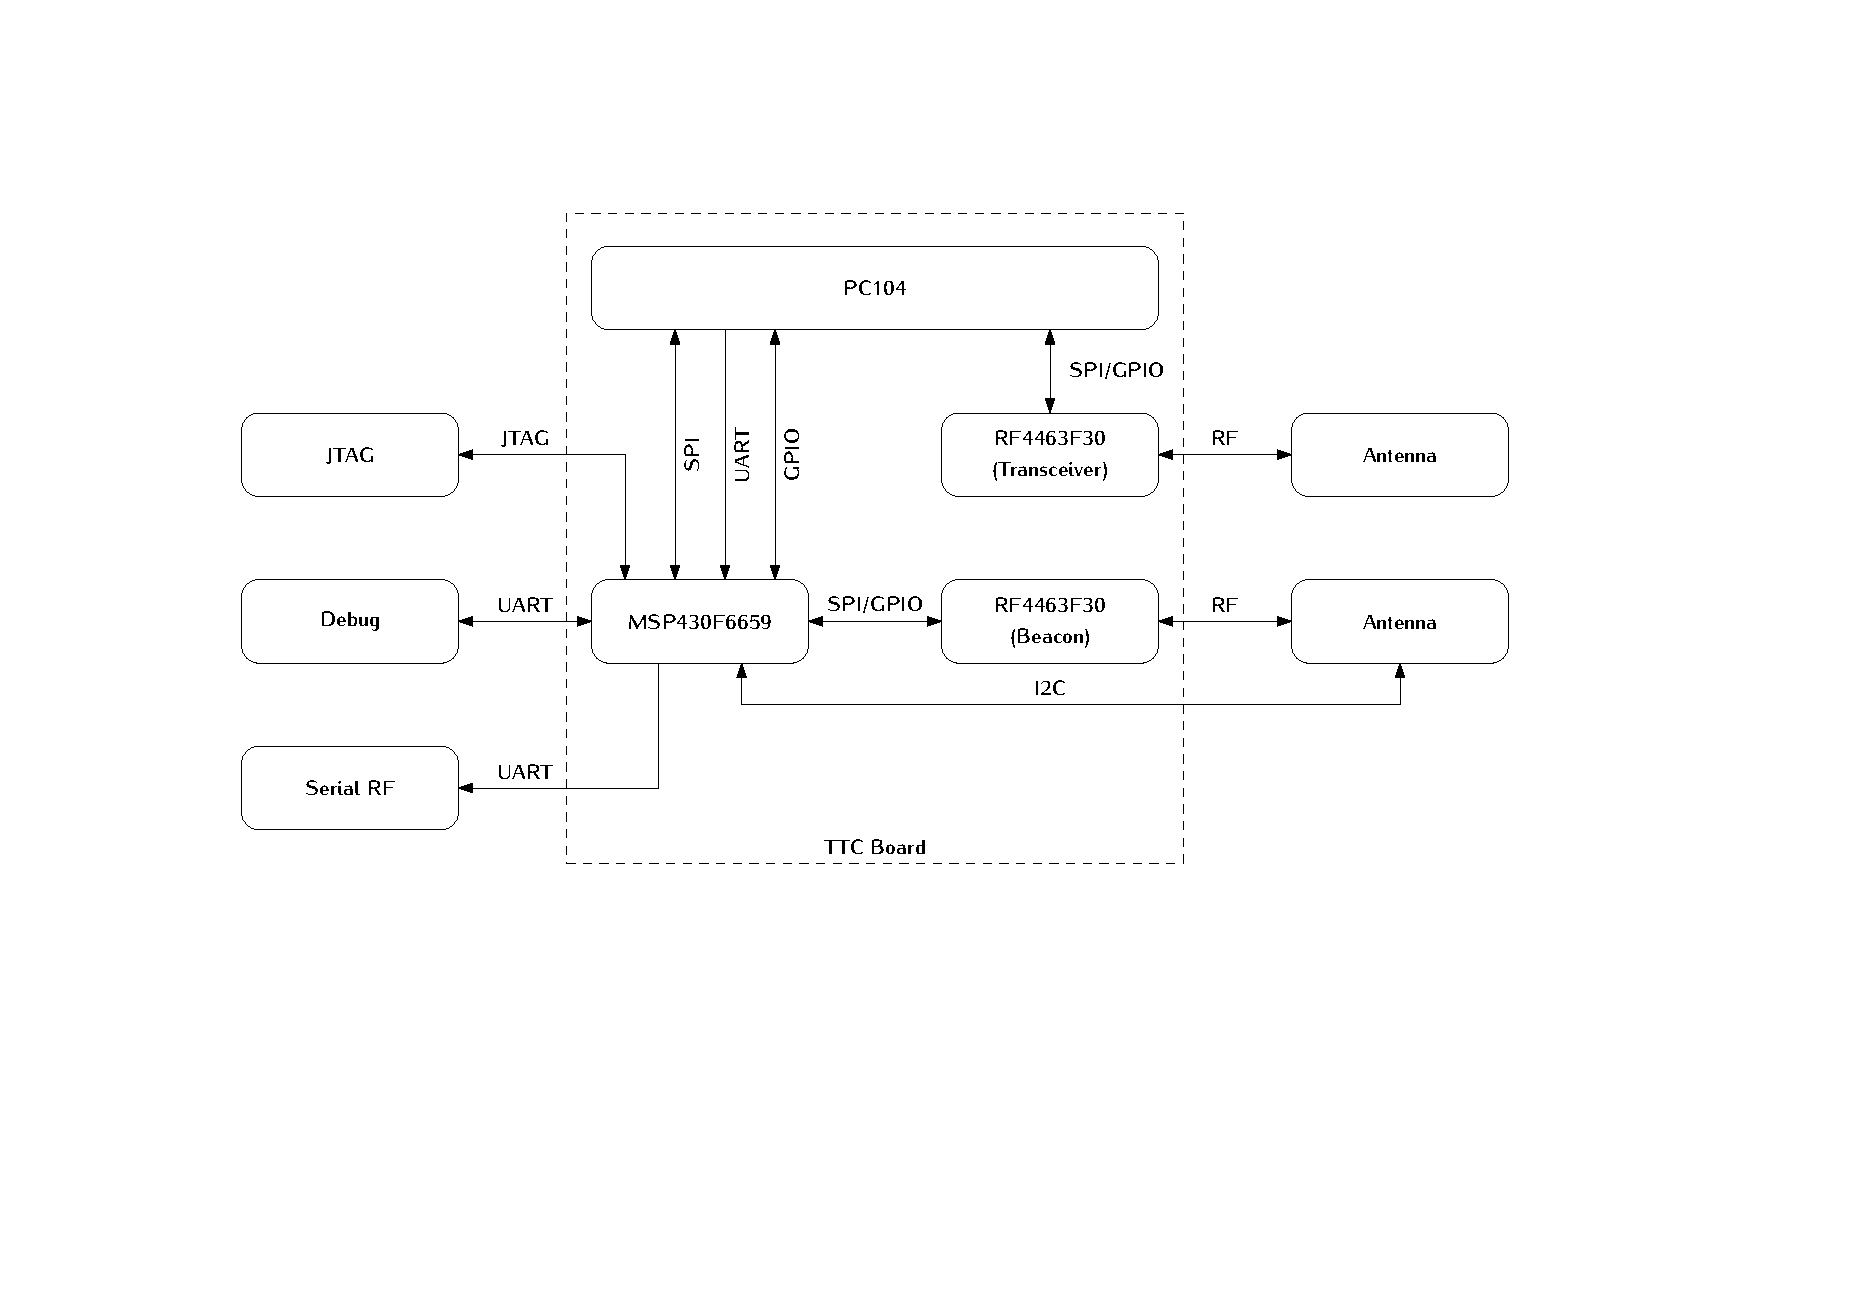
\includegraphics[width=\textwidth]{figures/hardware_diagram.pdf}
		\caption{Hardware diagram of the TTC module.}
		\label{fig:hardware-diagram}
	\end{center}
\end{figure}

\section{Main Components}

M...

\subsection{Microcontroller}

The beacon microcontroller is the MSP430F6659IPZR \cite{msp430f6659}. Its main characteristics can be found in the table \ref{tab:msp430f6659-info}.

\nomenclature{\textbf{CPU}}{Central Processing Unit.}
\nomenclature{\textbf{RAM}}{Random Access Memory.}
\nomenclature{\textbf{GPIO}}{General Purpose Input/Output.}
\nomenclature{\textbf{I$^{2}$C}}{Inter-Integrated Circuit.}
\nomenclature{\textbf{SPI}}{Serial Peripheral Interface.}
\nomenclature{\textbf{UART}}{Universal Asynchronous Receiver/Transmitter.}
\nomenclature{\textbf{DMA}}{Direct Memory Access.}
\nomenclature{\textbf{ADC}}{Analog-To-Digital Converter.}
\nomenclature{\textbf{BSL}}{Bootstrap Loader.}

\begin{table}[!h]
	\begin{center}
		\begin{tabular}{lc}
			\toprule[1.5pt]
			\textit{Characteristic} & \textit{Value} \\
			\midrule
			CPU & MSP430 \\
			Frequency & Up to 20 MHz \\
			Non-volatile memory & 512 kB \\
			RAM & 66 kB \\
			GPIO pins & 74 \\
			I$^{2}$C & 3 \\
			SPI & 6 \\
			UART & 3 \\
			DMA & 6 \\
			ADC & ADC12-12ch \\
			Comparators & 12 inputs \\
			Timers - 16-bit & 4 \\
			Multiplier & $32 \times 32$ \\
			BSL & USB \\
			Min $V_{cc}$ & 1,8 V \\
			Max $V_{cc}$ & 3,6 V \\
			Active Power & $360\ \mu A/MHz$ \\
			Standby Power (LMP3) & $2,6\ \mu A$ \\
			Wakeup Time & $3\ \mu s$ \\
			Operating Temperature Range & -40 to 80 $^{\circ}C$ \\
			\bottomrule[1.5pt]
		\end{tabular}
		\caption{MSP430F6659 features.}
		\label{tab:msp430f6659-info}
	\end{center}
\end{table}

\subsection{Radio Modules}

The NiceRF RF4463F30 \cite{rf4463f30} is a transceiver module based on the Silicon Labs Si4463 \cite{si4463} radio. This module also contains a PA module to increase the output power up to 31 dBm.

\subsubsection{Si4463}

\begin{table}[!h]
	\begin{center}
		\begin{tabular}{lcc}
			\toprule[1.5pt]
			\textit{Characteristic} & \textit{Value} & \textit{Unit} \\
			\midrule
			Frequency range & 119-1050 & MHz \\
			Receiver sensitivity & -126 & dBm \\
			Modulation & (G)FSK, 4(G)FSK, (G)MSK and OOK & - \\
			Max. output power & +20 & dBm \\
			PA support & +27 to 30 & dBm \\
			Ultra low current powerdown modes & 30 (shutdown), 50 (standby) & nA \\
			Data rate & 100 bps to 1 Mbps & - \\
			Power supply & 1,8 to 3,6 & V \\
			TX and RX FIFOs & 64 bytes for each or 129 bytes shared & - \\
			\bottomrule[1.5pt]
		\end{tabular}
		\caption{Si4463 features.}
		\label{tab:si4463-info}
	\end{center}
\end{table}

\section{External Connections}

This section describes the external available connections of the TTC module.

In the figure \ref{fig:connections-ref}, all the external connections are enumerated.

\begin{figure}[!h]
	\begin{center}
		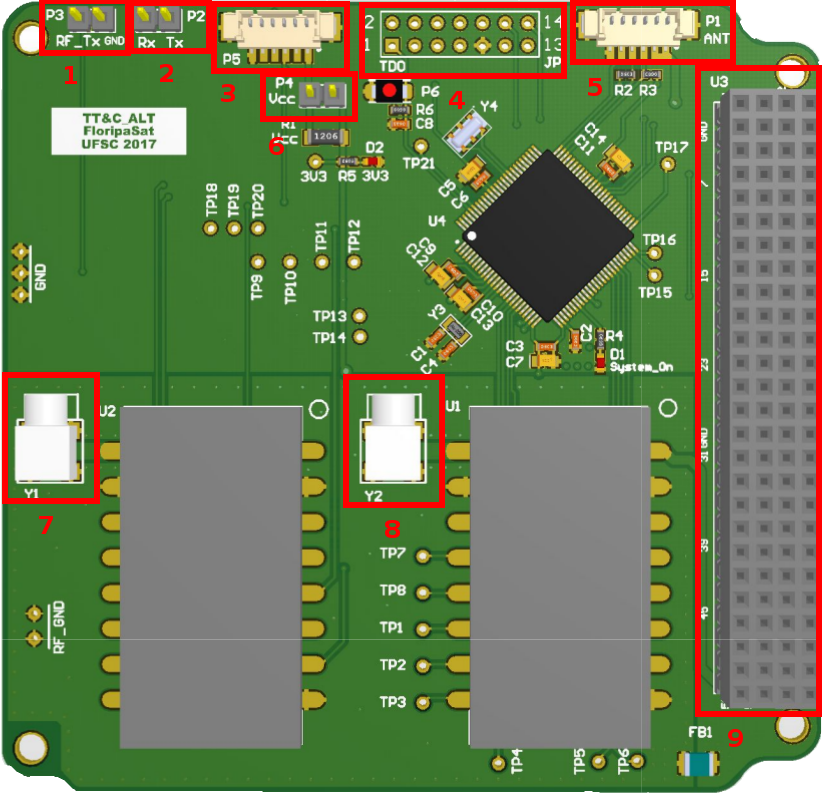
\includegraphics[width=0.75\textwidth]{figures/ttc_board_pins}
		\caption{External connections on the board.}
		\label{fig:connections-ref}
	\end{center}
\end{figure}

A brief description of each connection is presented in the table \ref{tab:connections-ref}.

\begin{table}[!h]
	\begin{center}
		\begin{tabular}{L{1.3cm} C{3cm} C{10cm}}
			\toprule[1.5pt]
			\textit{Number} & \textit{Connector} & \textit{Description} \\
			\midrule
			1 & Male pin header ($1 \times 2$) & UART TX $@$4800 bps. These pins transmit the beacon packets over a serial connection (It is enable in the configuration file, setting the BEACON\_RADIO variable as UART\_SIM). \\
			2 & Male pin header ($1 \times 2$) & Debug UART TX/RX $@$115200 bps. These pins transmit a description of the main events of the beacon software during it's execution. This feature is only available in DEBUG\_MODE. \\
			3 & Male PicoBlade$^{TM}$ ($\times 6$) & JTAG and Debug. This connection contains the relevant pins of the connectors 2 and 4. \\
			4 & Male pin header ($2 \times 2$) & MSP430 JTAG. This connection is for programming the uC code, using a MSP-FET debugger. \\
			5 & Male PicoBlade$^{TM}$ ($\times 6$) & Antenna I2C. I2C bus for a communication channel with the antenna module. \\
			6 & Male pin header ($1 \times 2$) & Power supply jumper. With a jumper, the beacon microcontroller power source comes from the JTAG connector. Without a jumper, the uC power supply comes from a pin of the PC104 connector. \\
			7 & Female Angled MCX & 437 MHz band RF signal (Goes to the antenna module). \\
			8 & Female Angled MCX & 145 MHz band RF signal (Goes to the antenna module). \\
			9 & Male/Female PCI-104 & PCI-104. Power supply and communication buses with others stacked up modules. \\
			\bottomrule[1.5pt]
		\end{tabular}
		\caption{External connections description.}
		\label{tab:connections-ref}
	\end{center}
\end{table}

The connections 1, 2, 4 and 6 were designed to be used during the software development stage, and not during the satellite operation.

\subsection{PCI-104 Pins}

The table \ref{tab:pci104-ref} describes the PCI-104 connector used pins. The first column is the row number of the connector, and the remaining columns are the respective columns (Named as H1A, H1B, H2A and H2B respectively). If the pin has no description, it is not connected to the TTC board.

\begin{table}[!h]
	\begin{center}
		\begin{tabular}{L{1cm} C{3cm} C{3cm} C{3cm} C{3cm}}
			\toprule[1.5pt]
			\textit{Row} & \textit{H1A} & \textit{H1B} & \textit{H2A} & \textit{H2B} \\
			\midrule
			1 & GND & GND & GND & GND \\
			2 & GND & GND & GND & GND \\
			3 & - & - & UART RX $@$4800 bps from the EPS module. & - \\
			4 & Telemetry radio GPIO0 & Telemetry radio GPIO1 & - & - \\
			5 & Telemetry radio GPIO2 & Enable beacon radio power supply & - & - \\
			6 & Telemetry radio SDN & - & OBDH communication (SPI MOSI) & OBDH communication (SPI clock) \\
			7 & - & - & OBDH communication (SPI chip select) & OBDH communication (SPI MISO) \\
			8 & - & - & - & - \\
			9 & - & - & - & - \\
			10 & - & - & - & - \\
			11 & - & - & - & - \\
			12 & - & - & - & - \\
			13 & - & - & - & - \\
			14 & - & - & Beacon uC power supply (3,3 V/50 mA) & 3,3 V beacon uC power supply (3,3 V/50 mA) \\
			15 & GND & GND & GND & GND \\
			16 & GND & GND & GND & GND \\
			17 & - & - & - & - \\
			18 & Telemetry radio SPI clock & - & - & - \\
			19 & Telemetry radio SPI MISO & - & - & - \\
			20 & Telemetry radio SPI MOSI & Telemetry radio SPI chip select & - & - \\
			21 & - & - & - & - \\
			22 & - & - & - & - \\
			23 & - & - & - & - \\
			24 & - & - & - & - \\
			25 & Telemetry radio power supply (5 V/500 mA) & - & - & - \\
			26 & Beacon radio power supply (5 V/500 mA) & - & - & - \\
			\bottomrule[1.5pt]
		\end{tabular}
		\caption{PCI-104 connector reference.}
		\label{tab:pci104-ref}
	\end{center}
\end{table}

%****************************************************
%****************************************************
%-- SOFTWARE ----------------------------------------
%****************************************************
%****************************************************

\chapter{Software}

\lettrine{S}{oftware}...

\nomenclature{\textbf{HAL}}{Hardware Abstraction Layer.}

\begin{figure}[!h]
	\begin{center}
		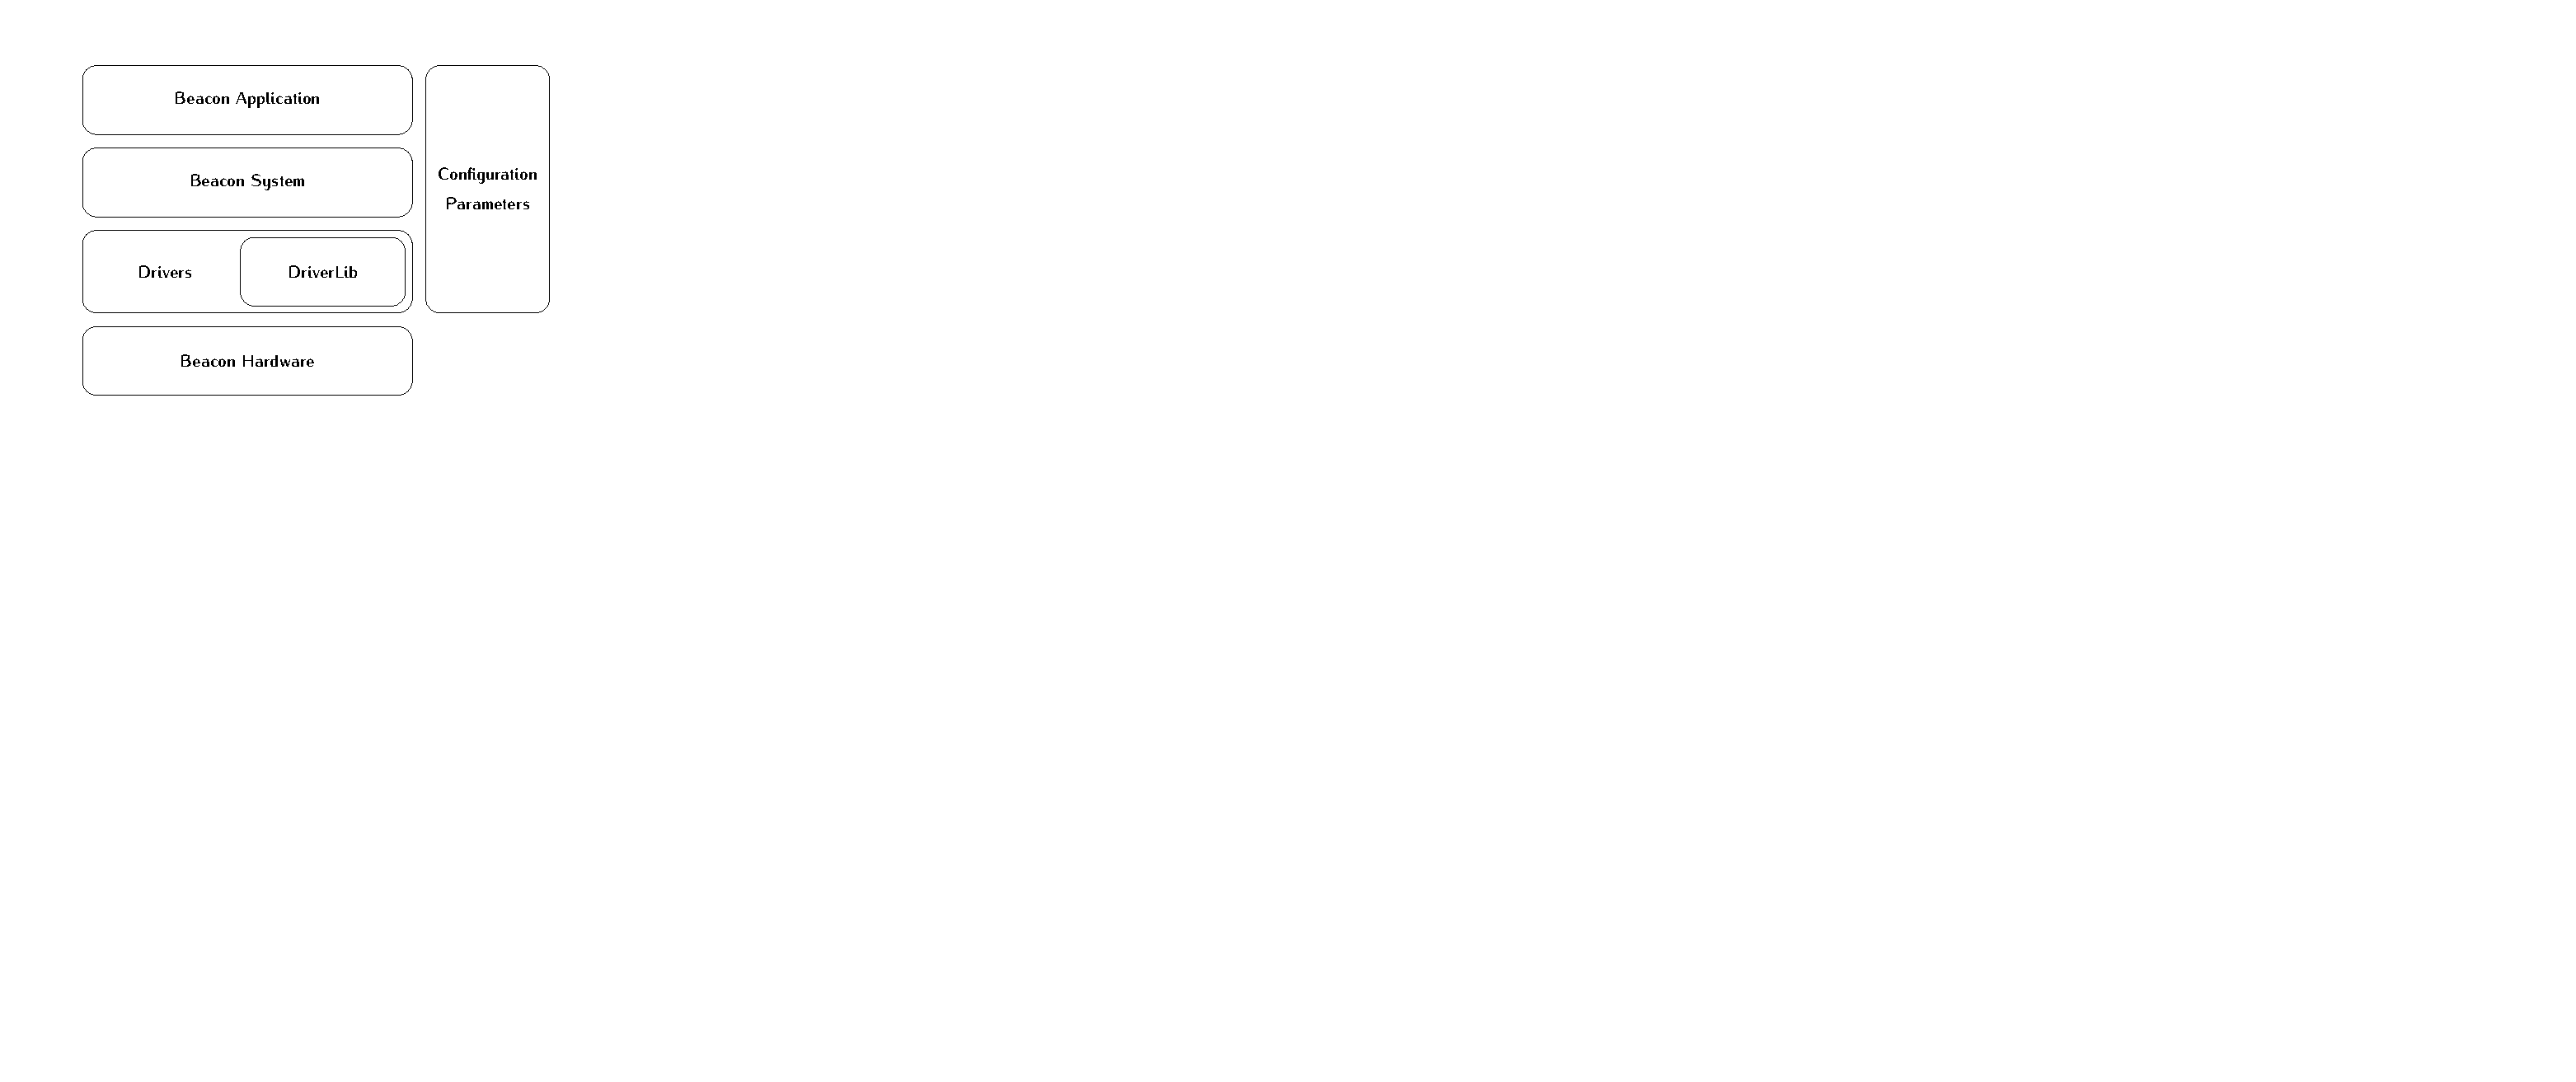
\includegraphics[width=0.5\textwidth]{figures/beacon_software_layers.pdf}
		\caption{Beacon software stack-up.}
		\label{fig:beacon-software-layers}
	\end{center}
\end{figure}

\section{Flowcharts}

\begin{figure}[!h]
	\begin{center}
		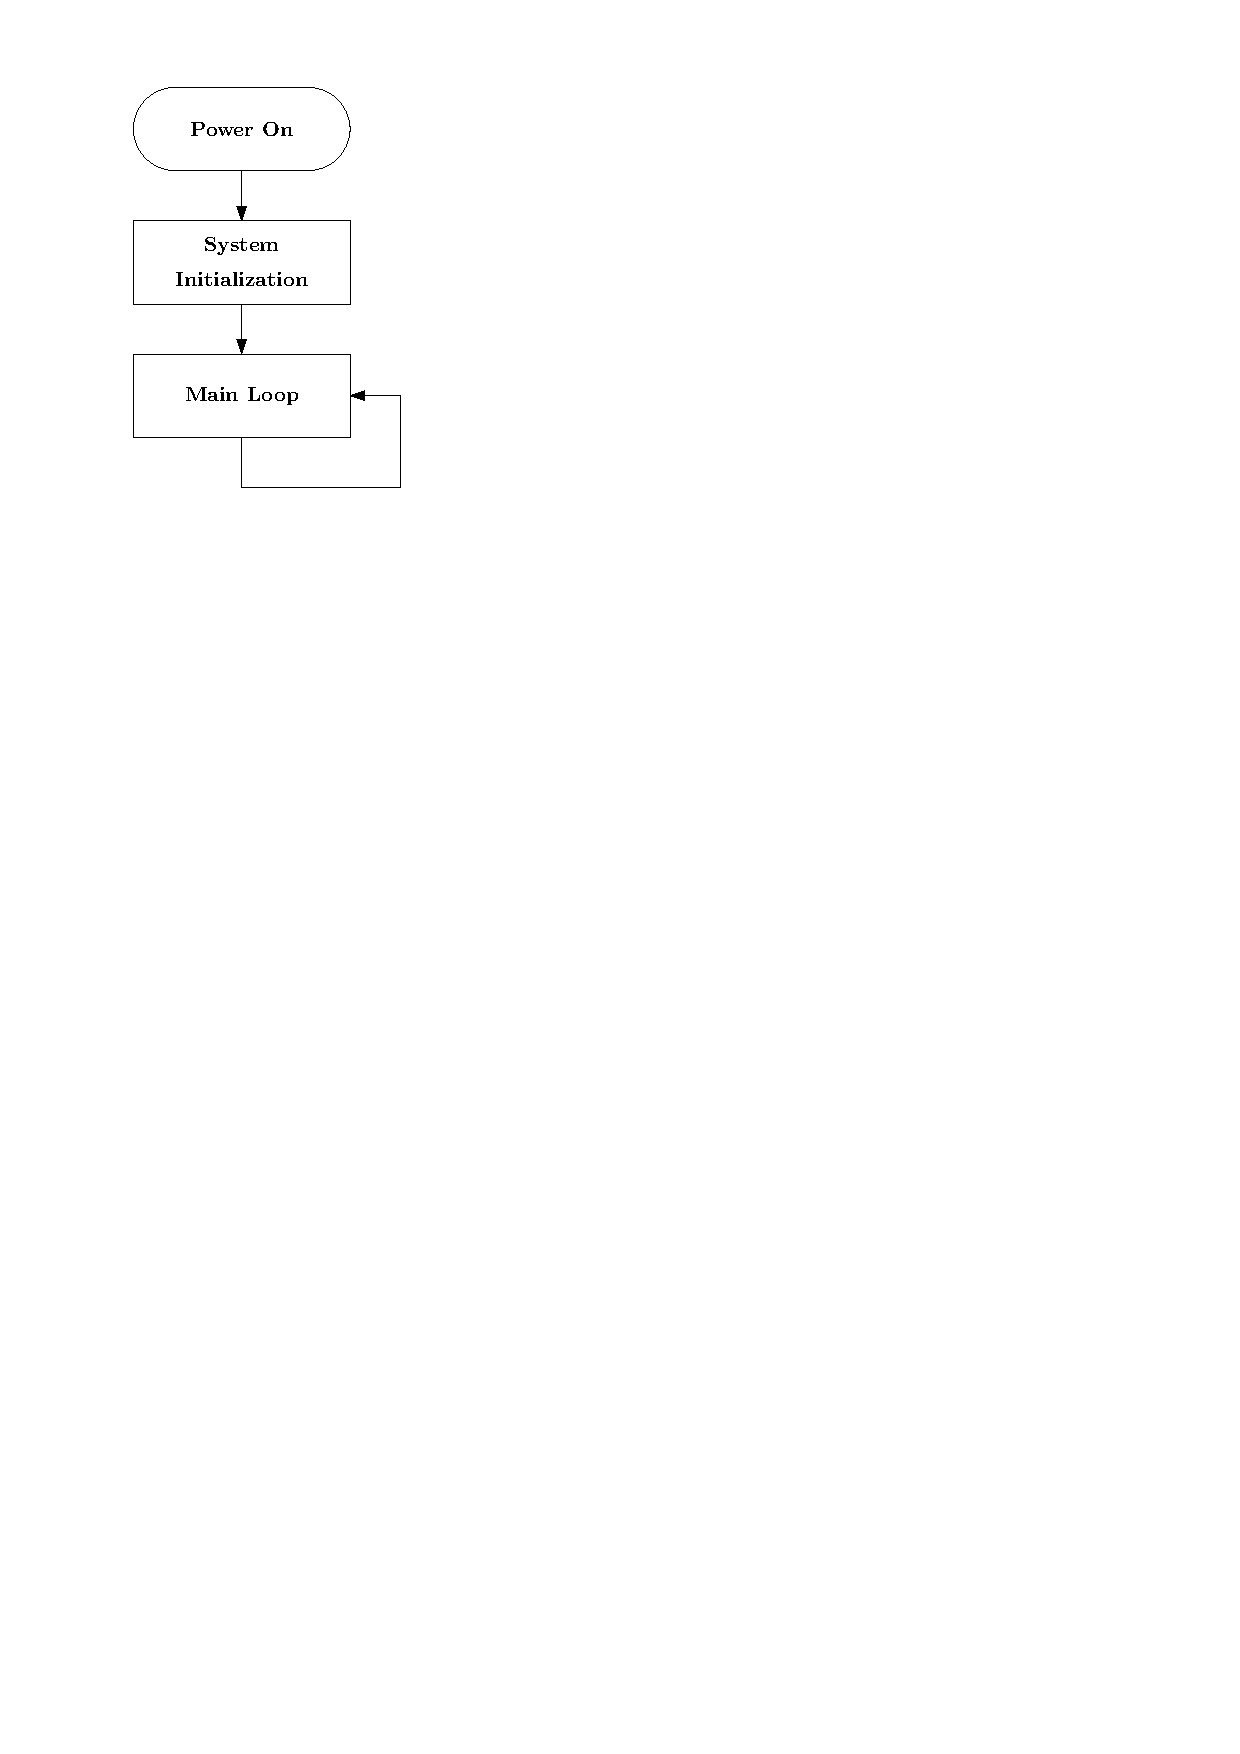
\includegraphics[width=0.25\textwidth]{figures/beacon_main_flowchart.pdf}
		\caption{Main flowchart of the beacon software.}
		\label{fig:beacon-main-flowchart}
	\end{center}
\end{figure}

\nomenclature{\textbf{ISR}}{Interruption Service Routine.}

\begin{figure}[!h]
	\begin{center}
		\subfigure[OBDH communication ISR flowchart.\label{fig:beacon-obdh-isr-flowchart}]{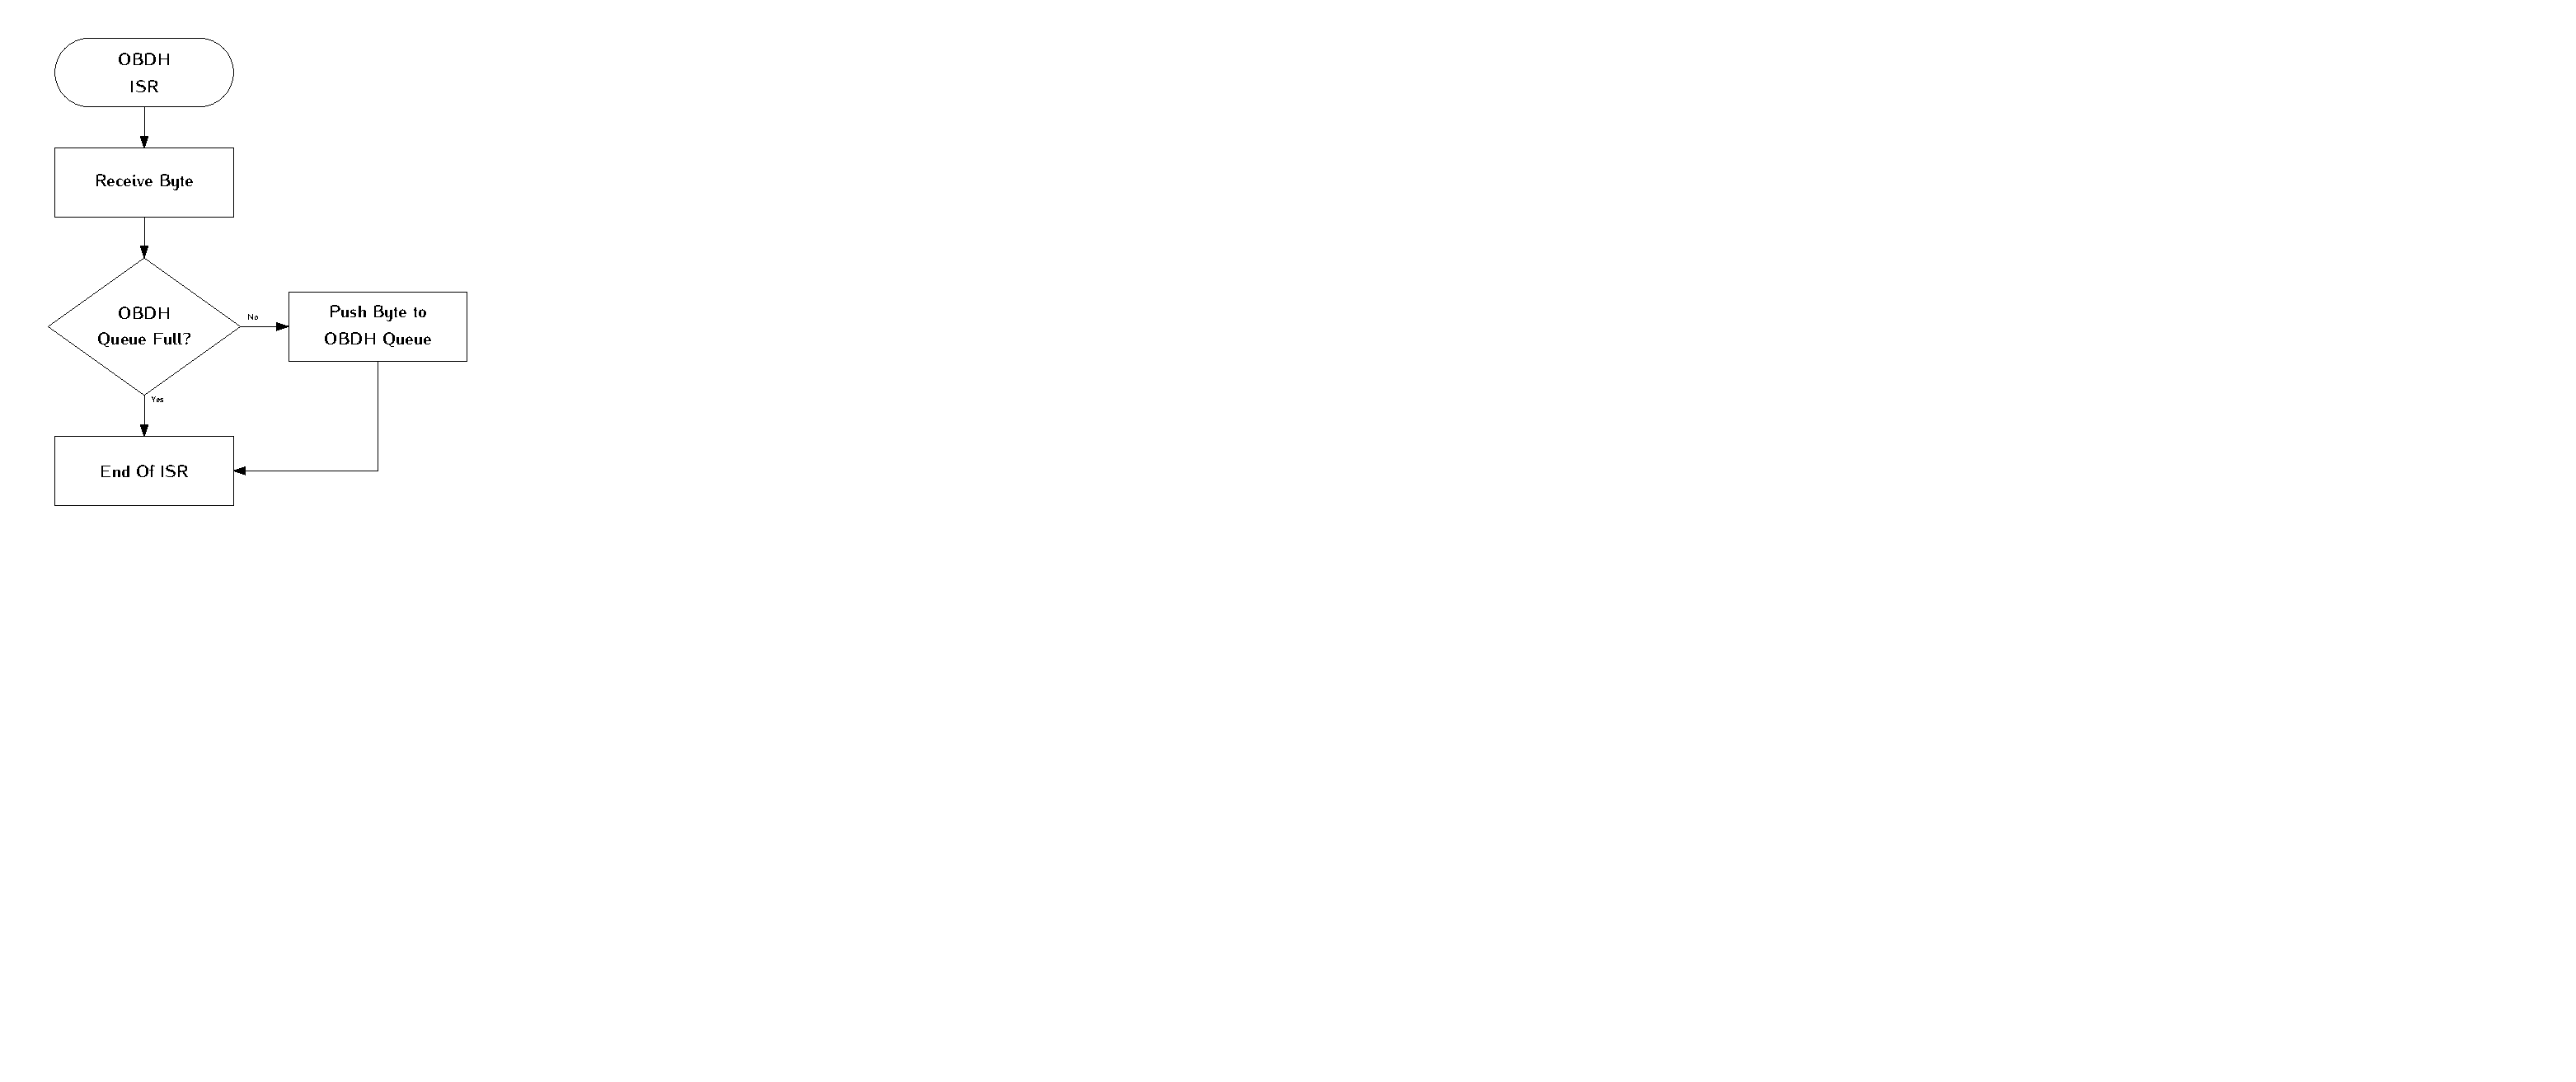
\includegraphics[width=0.4\textwidth]{figures/beacon_obdh_isr_flowchart.pdf}}
		\qquad
		\subfigure[EPS communication ISR flowchart.\label{fig:beacon-eps-isr-flowchart}]{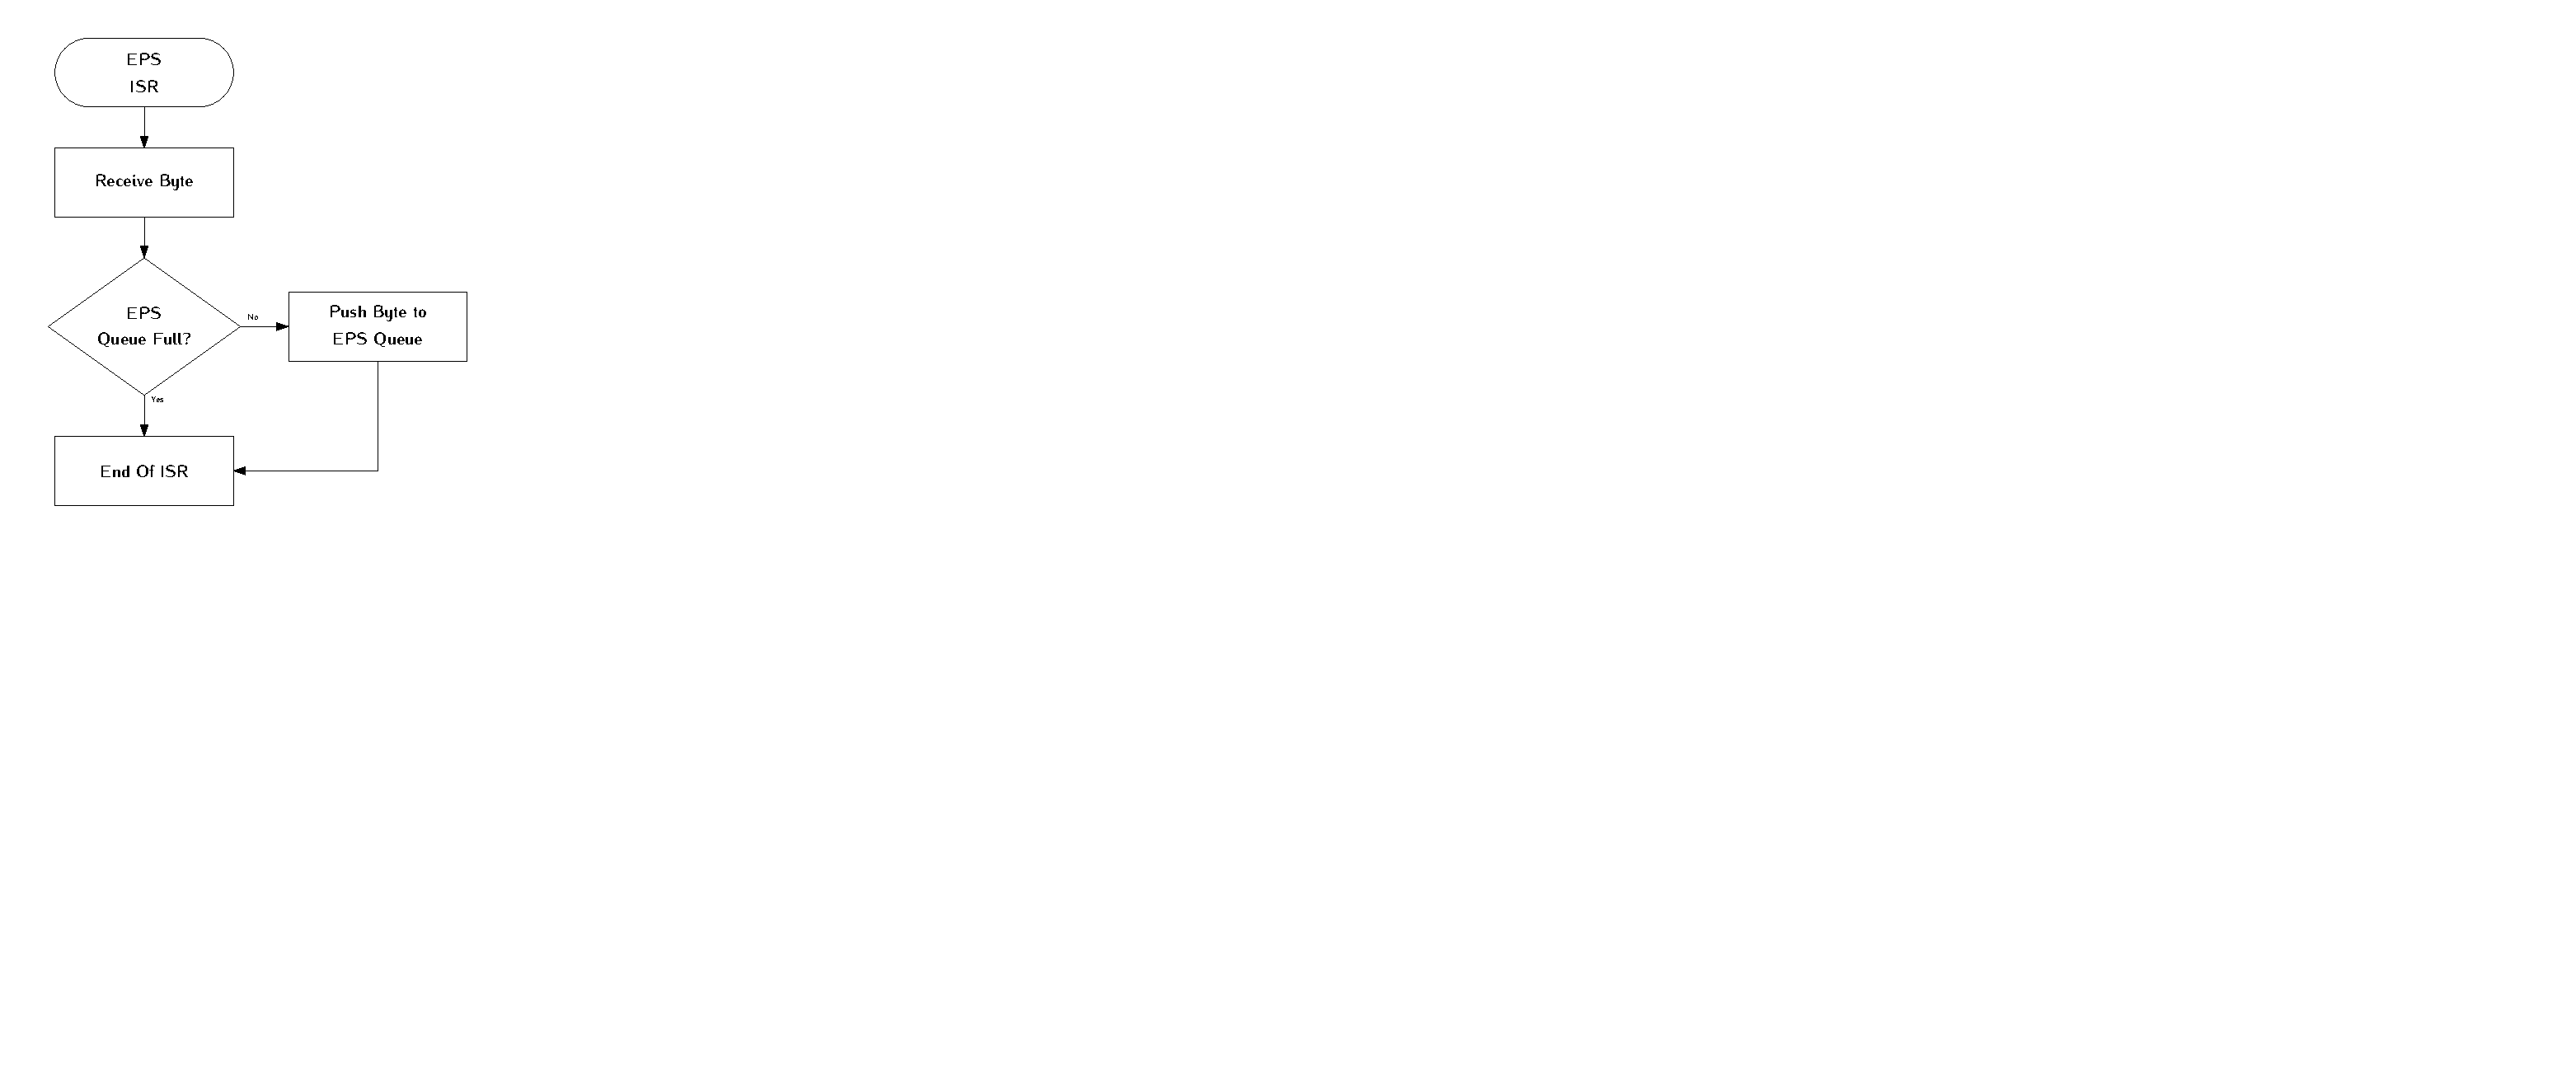
\includegraphics[width=0.4\textwidth]{figures/beacon_eps_isr_flowchart.pdf}}
		\caption{OBDH and EPS modules comunication ISRs routines.}
		\label{fig:obdh-eps-isr-flowchart}
	\end{center}
\end{figure}

%****************************************************
%****************************************************
%-- TESTS -------------------------------------------
%****************************************************
%****************************************************

\chapter{Tests}

\lettrine{T}{his}...

\section{RF Signal Power}

P...

%****************************************************
%****************************************************
%-- CONCLUSION --------------------------------------
%****************************************************
%****************************************************

\chapter{Conclusion} \label{ch:conclusion}

\lettrine{C}{onclusion}...

%****************************************************
%****************************************************
%-- REFERENCES --------------------------------------
%****************************************************
%****************************************************

\bibliography{references/site}
\addcontentsline{toc}{chapter}{Bibliography}

\end{document}
